% vim:ft=tex
\section{Simulation approach}
\label{sec:simulation}
In this section, we describe how our simulation is implemented, and how the 
implementation works. This is done in part to document our implementation, and 
in part to give the reader an overview of how our results are obtained.

Our simulation is implemented in the Python programming language, with the 
calculation intensive parts implemented in C for performance reasons. We 
assume a virtual coordinate system using meters as a base unit, and with the 
origin in the centre of the area we simulate. Each pedestrian (or actor) is 
described by a centre point and a radius, and each wall is described by a line 
segment connecting two points.

All parameters are stored as double precision floating point values where 
nothing else is indicated. We use custom data structures to keep track of the 
actors and walls while running the simulation. Python is used to set up the 
initial conditions, run the program's main control loop, and draw the 
simulation results through the \emph{PyGame} library \cite{pygame}. This 
allows to do both real-time animation as well as saving each simulation step 
to be assembled into a film afterwards. All calculations and data processing 
is done in a Python extension written in C, to increase performance. Gathering 
of data to draw the graphs and the drawing itself is done in the Python code 
as well. 

For all random numbers, the operating system's built-in random number 
generator is used and considered to be sufficient for our purposes. We run 
multiple simulations of the same initial conditions by fixing the seed of the 
random number generator to the same value for each run. Distributions are 
drawn by using the distribution functions of the \emph{NumPy} mathematical 
library for Python \cite{numpy}.

In this section we will describe briefly how the program is structured on a 
macro level, and go into more detail on the parts specific to the calculations 
of the model parameters. The full source code is available 
online\footnote{Source code hosted at Github: 
\url{https://github.com/tohojo/RUC-math--crowd-modeling}.}.

\subsection{Structure of the program}
The program is structured into four main parts: The simulation calculations, 
drawing of the simulations, plotting of parameters and the control part 
setting up parameters and calling the other parts as necessary. The drawing 
part mainly consists of a frontend to the drawing library, and so is not 
interesting to discuss here. The other parts will be described in the 
following, structured so as to present the sequence that is followed when a 
simulation is run. This description consists of three parts: setting up the 
simulation, calculations, and gathering of results.

\subsection{Setting up the simulation}
The program supports defining multiple \emph{scenarios} to simulate. Each 
scenario defines its own set of parameters, and a simulation run features one 
scenario. The parameters defined for each scenario include:

\begin{itemize*}
    \item The model constants, $A$, $B$, $U$, $\lambda$ and actor relaxation 
        time. These are the same for all actors in a simulation.
    \item Mean desired velocity and radius of actors and their standard 
        deviation, and the factor used to calculate the maximum velocity.
    \item The initial number of actors, the area(s) they start in and the 
        target(s) they move towards.
    \item The geometry of the scenario (i.e. placement of walls).
    \item Definition of the areas where measurement of data for plotting 
        graphs is done and which parameters should be plotted (see 
        section~\ref{sec:measurement}).
    \item Various parameters related to drawing of the simulation, maximum run 
        time and optional continuous inflow of actors.
\end{itemize*}

Parameters that are not set for each scenario, but are defined once for all 
simulations are:

\begin{itemize*}
    \item Time step size.
    \item Plotting data sampling frequency.
    \item Seed value for the random number generator.
\end{itemize*}

How the values of the parameters are determined is described in 
section~\ref{sec:init-cond}. From these parameters, the simulation is set up 
by initialising the calculation module and creating the actors.

The actors are created with an initial velocity of zero, and distributed 
randomly within the area(s) designated by the parameters for the scenario. To 
avoid having actors start out by overlapping, the starting area is divided 
into a grid with cells a little larger than the size of the maximum diameter 
of the generated actors. The actors are then placed into random cells of the 
grid. This makes the starting configuration of the actors a little more rigid 
than what might otherwise be observed, but we feel this is acceptable since 
actors move out of these grid cells within the first few time steps.

\subsection{Calculation of the model}
For each step of the simulation, the calculations are tun in two parts: 
Finding the accelerations (or resulting force) for all actors, and updating 
position and velocity for the actors.  Since the acceleration for each actor 
is dependent on both position and velocity of the other actors, splitting the 
calculations this way enables us to do the calculations of each actor in any 
order, and even parallel. The drawback is that the actors are only affected by 
the movement and positions of other actors as they were at the end of the last 
simulation step. This means that the time step has to be small enough that 
this doesn't matter in practice.

The acceleration vectors for each actor, $\alpha$, is calculated in three 
steps, corresponding to the parts $\overrightarrow{f_\alpha^0}$, 
$\overrightarrow{f_{\alpha \beta}}$ and $\overrightarrow{f_{\alpha B}}$ from 
section~\ref{sec:the-model}. In each simulation step the three forces are 
calculated in order, first calculating the desired force, then the repulsive 
force from each of the other actors in the simulation, and finally the 
repulsive force from each wall. The resulting vectors are added to yield the 
total acceleration for each actor.

After this is calculated for all actors, their velocities and positions are 
updated in a separate step. Each of these four steps are described in detail 
in the following. The code calling the other parts of the calculation can be 
seen in code listing~\ref{lst:calling}. This function is called once for each 
actor (index \texttt{i}) for each simulation step.

\begin{lstlisting}[caption={Code calling the other parts of the 
    calculation.},label=lst:calling]
void calculate_forces(Py_ssize_t i)
{
    int j;
    add_desired_acceleration(&actors[i]);

    for(j = 0; j < a_count; j++) {
        if(i == j) continue;
        add_repulsion(&actors[i], &actors[j]);
    }

    add_wall_repulsion(&actors[i]);
}
\end{lstlisting}

\subsubsection{Calculating the desired force}
The function for calculating the desired force can be seen in code 
listing~\ref{lst:desired-force}. Of note is the implementation on lines 7-19 
of the conditional definition of $V_\alpha^0(t)$ given in 
equation~\eqref{eqn:cond-define} and the creation of a unit vector in lines 
20-21 to add the direction to the desired velocity.

To increase performance, it is preferred to update values in place, instead of 
copying them around in different places of the computer's memory. This gives 
rise to the constructs around the \texttt{vector\_i*}-functions in the code; 
here the \emph{i} stands for ``in place''.

\begin{lstlisting}[caption={Code for calculating the desired 
    force.},label=lst:desired-force]
static void add_desired_acceleration(Actor * a)
{
    double average_velocity = 0.0, impatience = 0.0, 
           desired_velocity = 0.0;
    Vector desired_direction = {0.0, 0.0};

    if(a->time) {
        double proj = vector_projection_length(
                a->initial_position, a->target, a->position);
        average_velocity = proj / a->time;

        impatience = 1.0 - average_velocity / a->initial_desired_velocity;

        desired_velocity = (1.0-impatience) * a->initial_desired_velocity + \
                           impatience * a->max_velocity;

    } else {
        desired_velocity = a->initial_desired_velocity;
    }
    desired_direction = vector_sub(a->target, a->position);
    vector_unitise(&desired_direction);

    a->acceleration = vector_mul(desired_direction, desired_velocity);
    vector_isub(&a->acceleration, &a->velocity);
    vector_imul(&a->acceleration, 1.0/a->relax_time);
}
\end{lstlisting}

\subsubsection{Repulsion from other actors}
The two functions used for calculating the repulsion from other actors is seen 
in code listing~\ref{lst:actor-repulsion}. The \texttt{add\_repulsion} function 
is called for each pair of actors. The force without any angle dependency is 
calculated in the \texttt{calculate\_repulsion} function, and is modified by 
the angular dependence if the actor's velocity is not zero, and $\lambda$ is 
not one. If the velocity is zero, calculating the dot product would result in 
a division by zero, and if $\lambda$ is one, modifying the force by the 
angular dependence would have no effect. The whole calculation is skipped if 
one of the constants $A$ or $B$ are zero, as this would make the calculations 
have no effect, or result in a division by zero, respectively.

\begin{lstlisting}[caption={Calculating the repulsion from other 
    agents.},label=lst:actor-repulsion]
Vector calculate_repulsion(Actor * a, Actor * b, double A, double B)
{
    double radius_sum = a->radius + b->radius;
    Vector from_b     = vector_sub(a->position, b->position);
    double distance   = vector_length(from_b);

    vector_unitise(&from_b);
    vector_imul(&from_b, A * exp((radius_sum-distance)/B));

    return from_b;
}

void add_repulsion(Actor * a, Actor * b)
{
    if(!A || !B) return;
    Vector repulsion = calculate_repulsion(a, b, A, B);
	if(a->velocity.x && a->velocity.y && lambda < 1.0) {
		Vector from_b = vector_sub(b->position, a->position);

		double cosine = vector_dot(a->velocity, from_b)/(
				vector_length(a->velocity) * vector_length(from_b));

		vector_imul(&repulsion, (lambda + (1-lambda)*((1+cosine)/2)));
	}
    vector_iadd(&a->acceleration, &repulsion);
}
\end{lstlisting}

\subsubsection{Repulsion from walls}
The code for adding the repulsion from the walls is shown in code 
listing~\ref{lst:wall-repulsion}. The \texttt{add\_wall\_repulsion} function 
is called for each actor and consists of two parts: Finding the points on the 
walls where repulsion should be calculated from, and calculating the repulsion 
from these points. The force from the repulsion points is calculated in the 
function \texttt{calculate\_wall\_repulsion} that is called for each repulsion 
point. This calculation corresponds to equation~\eqref{eqn:wall-repulsion}.

\begin{lstlisting}[caption={Code to calculate the repulsion from the 
    walls.},label=lst:wall-repulsion]
void add_wall_repulsion(Actor * a)
{
    int i;
    Vector * repulsion_points  = PyMem_Malloc(w_count * sizeof(Vector));
    int rep_p_c = 0;
    Vector repulsion;

    rep_p_c = find_repultion_points(a, repulsion_points);

    for(i = 0; i < rep_p_c; i++) {
        repulsion = calculate_wall_repulsion(a, repulsion_points[i]);
        vector_iadd(&a->acceleration, &repulsion);
    }


    PyMem_Free(repulsion_points);
}

Vector calculate_wall_repulsion(Actor * a, Vector repulsion_point)
{
    Vector repulsion = {0,0};
    Vector repulsion_vector = vector_sub(repulsion_point, a->position);
    double repulsion_length = vector_length(repulsion_vector);

    repulsion.x = U * (1/a->radius) * \
                  (exp(-repulsion_length/a->radius)*\
                   (a->position.x-repulsion_point.x))/repulsion_length;
    repulsion.y = U * (1/a->radius) * \
                  (exp(-repulsion_length/a->radius)*\
                   (a->position.y-repulsion_point.y))/repulsion_length;

    return repulsion;
}
\end{lstlisting}

The function for finding the repulsion points on the walls is seen in code 
listing~\ref{lst:repulsion-points}. This is an implementation of the algorithm 
described in section~\ref{sec:repulsion-points}. Lines 9-27 corresponds to 
step one in the algorithm description that identifies definite repulsion 
points (those that are not wall endpoints) and possible repulsion points 
(those that are endpoints).

In lines 29-35 an endpoint is discarded if it is already used because it is 
shared with a wall that has already defined a repulsion point. In lines 36-57 
endpoints that are not discarded in this way are added to the list of 
repulsion points if they are either not free-floating (i.e. shared with 
another wall), or closer to the actor centre than the actor's radius. This 
ensures that doorways to not repulse actors that are passing through it.

\begin{lstlisting}[caption={Code for finding the wall repulsion 
    points.},label=lst:repulsion-points]
int find_repultion_points(Actor * a, Vector repulsion_points[])
{
    int i,j;
    double projection_length;
    Vector * used_endpoints     = PyMem_Malloc(2*w_count * sizeof(Vector));
    Vector * possible_endpoints = PyMem_Malloc(w_count * sizeof(Vector));
    int rep_p_c = 0, use_e_c = 0, pos_e_c = 0;

    for(i = 0; i < w_count; i++) {
        Wall w = walls[i];
        projection_length = vector_projection_length(w.start, w.end, a->position);
        if(projection_length < 0)  {
            possible_endpoints[pos_e_c++] = w.start;
        } else if(projection_length > w.length) {
            possible_endpoints[pos_e_c++] = w.end;
        } else {
            // We have the length, L, of how far along AB the projection point is.
            // To turn this into a point, we multiply AB with L/|AB| and add
            // this vector to the starting point A.
			// P = A + AB*L/|AB|
            repulsion_points[rep_p_c++] = vector_add(w.start, 
                    vector_mul(vector_sub(w.end, w.start), 
                        projection_length/w.length));
            used_endpoints[use_e_c++] = w.start;
            used_endpoints[use_e_c++] = w.end;
        }
    }

    for(i = 0; i < pos_e_c; i++) {
        int use_e = 1;
        for(j = 0; j < use_e_c; j++) {
            if(vector_equals(possible_endpoints[i], used_endpoints[j])) {
                use_e = 0;
            }
        }
        if(use_e) {
			// Keep track of whether the endpoint is free-floating, i.e. if
			// it is shared with another wall.
			int free_e = 1;
			for(j = 0; j < pos_e_c; j++) {
				if(i != j && 
						vector_equals(possible_endpoints[i],
							possible_endpoints[j])) {
					free_e = 0;
				}
			}
			// Endpoints that are free-floating (i.e. sides of doorways) are
			// only considered for repulsion if they are closer to the actor
			// than the actor's radius. This allows actors to pass more
			// freely through doorways.
			if(!free_e || 
					vector_length(vector_sub(a->position,
							possible_endpoints[i])) < a->radius) {
				repulsion_points[rep_p_c++] = possible_endpoints[i];
				used_endpoints[use_e_c++] = possible_endpoints[i];
			}
        }
    }

    PyMem_Free(used_endpoints);
    PyMem_Free(possible_endpoints);

    return rep_p_c;
}
\end{lstlisting}

\subsection{Updating position and velocity}
After every actor has been updated with a resulting acceleration vector from 
the current simulation step, all actors update their position and velocity.  
The position is updated by calculating a displacement vector as follows:

\begin{equation}
    \Delta p = (v_x \Delta t + \frac{1}{2}a_x \Delta t^2, v_y \Delta t + 
    \frac{1}{2}a_y \Delta t^2)
\end{equation}
% TODO: Viggo had question marks around parts of this equation. Look into why.

Where $v_x$ and $v_y$ are the $x$ and $y$ components of the velocity vector, 
$a_x$ and $a_y$ are the $x$ and $y$ components of the acceleration vector, and 
$\Delta t$ is the time step.

After updating the position, the actor's velocity is updated by adding the 
acceleration vector, to be used for the next simulation step. The code that 
does this is seen in code listing~\ref{lst:update-position}. Lines 14-19 are 
related to the measuring of data for plotting, and will be explained in 
section~\ref{sec:measurement}.

\begin{lstlisting}[caption={Code updating the actor 
    position.},label=lst:update-position]
void update_position(Actor * a)
{
    Vector delta_p;

    delta_p.x = a->velocity.x * timestep + 0.5 * a->acceleration.x * pow(timestep, 2);
    delta_p.y = a->velocity.y * timestep + 0.5 * a->acceleration.y * pow(timestep, 2);


    vector_iadd(&a->position, &delta_p);
	a->velocity = vector_add(a->velocity,
			vector_mul(a->acceleration, timestep));
    a->time += timestep;

	if(a->flowline_time < 0) {
        if(vector_projection_distance(
					flowline[0], flowline[1], a->position) < a->radius) {
			a->flowline_time = a->time;
		}
	}
}
\end{lstlisting}

% start parameters: p_n, v_n for each person.
% p for each wall
%
% steps:
%
% for each person:
%   calculate acceleration from the force parts of the model
%
% for each person:
%   update position by displacement vector
%       delta-p = (v_x*delta-t+1/2*a_x*delta-t^2, 
%       v_y*delta-t+1/2*a_y*delta-t^2)
%   update velocity for next step
%
%
% initial parameters:
%   Set using some sort of distribution around a mean
%
%
% constants:
%   Where do they come from?

\subsection{Measurement of the concepts flow rate, density and efficiency}
\label{sec:measurement}
We want to have some concepts we can use to compare the simulations and to see 
if the simulations make sense.  In this section we will describe how we want 
to measure the concepts efficiency, flow rate and density.

\textbf{Efficiency}
We will measure the efficiency throughout the simulations. The efficiency is a 
dimensionless number given by the average speed of each pedestrians divided by 
the desired speed of each pedestrian. We will meassure the avereage speed in each 
timestep as:

\begin{equation}
	\overline{V_t}=\frac{1}{N}\sum_{i=1}^{N}V_i
\end{equation}
Where $V_i$ is the speed of the i'th pedestrian and N is the number of pedestrians 
still left in the simulation(Since there is no reason to include pedestrians who have 
reach there desired point since they are not moving). Then to find the efficiency for 
the entire simulation we make a summation of $V_t$ for each time step and then divide 
with the number of simulation steps. So given as an equation we have

\begin{equation}
		E=\frac{1}{T}\sum_{t=0}^{T}\frac{\overline{V_i}}{V^0_{i}}
\end{equation}

Where T is the number os simulations step and $V^0_{i}$ is the desired speed. This will 
give us an meassure about how fast the avereage speed the pedestrians where moving. In 
crowed simulations one should expect the efficiency to go to zero since people won't move 
fast and in a low density simulations it should be expected to have a value close to one $1$. 
The efficiency will in some way be a more general measurement of how fast pedestrians move 
throug a simulation than say the time it takes for the pedestrias to leave a room. Because 
the time will be strongly depenten on the shape of the area in the simulation and will be 
hard to compare with another situation. 
	
\textbf{Flow rate}
Part of the model geometry was made as a line seqment where we measure the average flow 
rate and the maximum flow rate, as pedestrians crossing the line seqment per second. 
This line should of course be placed somewhere the pedestrians actually are moving through. 
So in the case of a squared room you could place the line in the doorway that people move 
through when leaving the room. Also you could place more than one line and see if there is 
a difference in the flow rate throughout the room.   When we meassure it we will againg have 
to be carefull with the time onwhich we meassureit. The time step length that we have chosen 
to use in the simulations is $0.01$s. This is very small when meassuring the flow rate because 
the pedestrians will be more than $0.1$s about crossing a line completly(I.e. a pedestrian 
with a radius of $0.4m$ will move at a speed of $40$m$/$s if he where to cross the line in 
one time step). So in many step the flow rate would then be zero and then suddenly $100 s^{-1}$ 
when just one pedestrian has crossed the line. On the other hand it would be just as bad to 
meassure it every time 20 second has gone since all the pedestrian might have crossed the 
line and maybe they did it in only 10 seconds. So it is important to choose the right time 
when meassuring the flowrate. We have chosen to measure it for each second, that is every 
time we have done $100$ time steps. This requires a pedestrian to move at $0.4m/s$ to 
entirely cross the line. Also we will calculate the flow speed for the entire simulation. 
This we will measure as the number of pedestrians who have crossed the line in the time 
that it took for the last pedestrians to cross the line.      
	
\textbf{Density}
Another thing that we want to measure is the density of the pedestrians. When we do this, 
it of course makes no sence to measure the density of the entire area we make the simulation 
on, because then it will only change when a pedestrian leaves the simulated area. What we will 
do to makes is usefull is that we will choose a certain area on wich we will measure the density. 
In the case of a squared room it would be intersting to measure on an area of a couple of square 
meters just before the door that the pedestrians are leaving through. A sketch of this can be seen 
on figure\ref{fig:density}   
	
 \begin{figure}
 \centering
 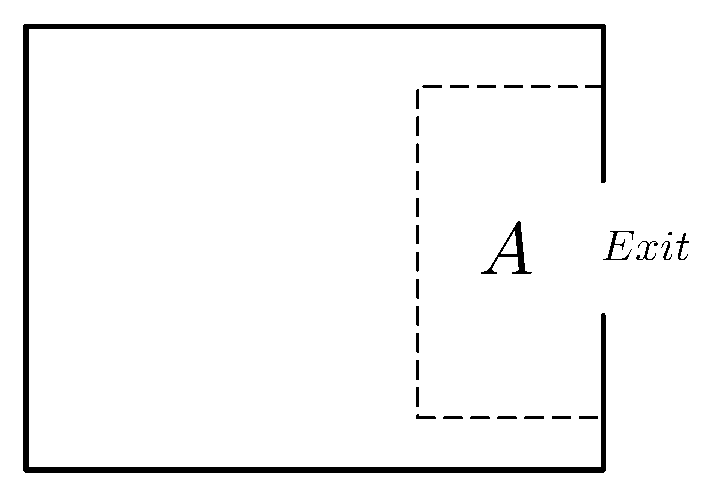
\includegraphics[scale=.5]{Figures/SquareCase.pdf}
 \caption{Here is a sketch of the area that we want to measure the density on when simulating a squared room.}
 \label{fig:density}
 \end{figure}

So when we do the measurement it will be given as the area covered by the pedestrian 
divided by entire area on wich we measure the density. So the density will, as the 
efficiency, be a nondimensional number. Is will give us a more precise density than 
if we measured the number of pedestrian in the same area.  Becuase the pedestrians 
who are standing on the edge of the area but not completly inside, will notaffect 
the density. The measure of the density we will use to compare with the flow rate 
an see if the two are correlating when doing a simulation. It would be expected 
that when the flow rate goes down the diensity goes up in value. But it could be 
interesting to see it it i the same an se if there is some linearity between the 
two. This of coures implies that the area we choos will also be where we put the 
line that the pedestrians will cross when measuring the flow rate.   

\subsection{Simulating our cases}
In this section we describe the geometrical features of our two cases, how many pedestrians we want in the simulations,
where the seqment line from which we measure the flow rate, the square used to measure the density and the describing the 
parameters used and how we want to modify them from simulation to simulation.

In case one we simulate agents leaving a squared room with the size 10 m x 10 m and with one exit with the size 1 m in the middle of
one of the wall seqments. The waypoint the agents are following is placed 3 meters from the exit outside the room.
The line seqment used to measure the flow rate is 2 m wide and placed outside the room with a distance of 0.3 m,
from the exit, to prevent that agents that are clogging are not measured more than one time.
The square used to measure the density has the size 2 m x 2 m, and is placed right in the room right in front of the exit.
We simulate the room with 100 pedestrians starting at random places and their initial velocity 0 m/s.
The agents desired velocity is Gaussian distributed around 1.36 m/s with a standard deviation of 0.26 m/s.
Maximum desired velocity is determined by multiplying the agents desired velocity with 1.3, so that the agents
maximum velocity and their desired velicity are linked.
$\lambda$ is initially set to 0.1, such that the agent are more influenced of what is going on in front of them.
The parameters A and B are set to respectively 2.2 and 0.2, and the relaxation time is set to 1.

In case two we simulate agents walking in both directions along a corridor of the size 50 m long and 4 m wide.
The agents are divided into two groups, each one starting in each end of the corridor, where the waypoint that the
left side group is following is placed 50 m behind the right end of the corridor. Correspondingsly the waypoint
the right side group is following is placed 50 m behind the left end of the corridor.
The seqment line we use to measure the flow rate with is placed in the middle of the corridor and is 4 m wide going from wall to wall.
The area used to measure the density is placed in the middle of the corridor, is 1 m long and 4 m wide and hence
also going from wall to wall.
In this simulation we start with 50 placed randomly on the right side of the line seqment used to measure the flow rate,
and 50 agents placed randomly on the left side of the line seqment.
The initial conditions are the same as in case one.
When the simulation has begun we do not want the simulation to stop when the agents have passed each other, therefore we
make two agent appear randomly on each half of the corridor each second in 60 second.

We want to simulate the two cases several times, where we vary one of the parameters at a time, to see if that improves the simulation,
in the sense that it looks more realistic, or that the flow rate, efficiency or density is the like of what \cite{self-org} simulated.
After the first simulation of each case with the initial conditions, we run some simulations where we change the parameter A and vary
it between 0.001 and 10.000.
Then we set A to the initial condition while we run some simulations where we change the parameter B and vary it between 0.001 and 10.000.
$\lambda$ is then varied between 0.100 and 1.000 while the other parameters are set to the initial conditions.
Some runs are made where $v^{max}_{\alpha}$ varies between 1.000 and 10.000.
The relaxation is varied between 0.100 and 10.000 and the timestep....
In case two we make some simulations where we vary the width of the door, between 0.700 and 1.000.
